\section{Single-Purpose-Web-App: Lunchapp}
\label{section:lunchapp}

\subsection{Beschreibung}

%- Was ist die Idee einer single purpose app -> bitte mit glossareintrag für single purpose app (bei fragen an sebbel wenden)
%- Das es ne Lunchapp wird erst unter Weiteres Vorgehen Beschreiben
%- siehe 5. semester word dokument

Bei diesem Prototyp handelt es sich um die Ausarbeitung einer \gls{glos:single_purpose_web_app}. Diese soll einen relevanten Inhalt, wie den Schichtplan oder das Lunchmenü, für die Mitarbeiter bereithalten. Somit ist ein Anreiz für die Mitarbeiter gegeben, diese Webseite aufzurufen. Auf dieser Seite soll ein Banner zu der Umfrage führen. Dieses soll dabei schlicht und nicht zu aufdringlich wirken, aber trotzdem die Aufmerksamkeit des Nutzers wecken. Klickt man auf das Banner, so gelangt man zur Umfrage. Um die relevanten Informationen zu schützen, könnte man einen Authentifizierungsmechanismus einrichten. Damit wird bezweckt, dass Mitarbeiter nur die für sie bestimmten Informationen, wie den Schichtplan, einsehen können. Durch diese Authentifizierung braucht sich der Mitarbeiter auch bei der Umfrage nicht mehr zusätzlich anmelden, sondern wird direkt vom System eingeordnet.

\subsection{Mockups}

Abbildungen \ref{wamu1} bis \ref{wamu3} zeigen drei verschiedene Design-Mockups, die wir für die Single-Purpose-App entwickelt haben:

\begin{figure}[H] 
\centering 
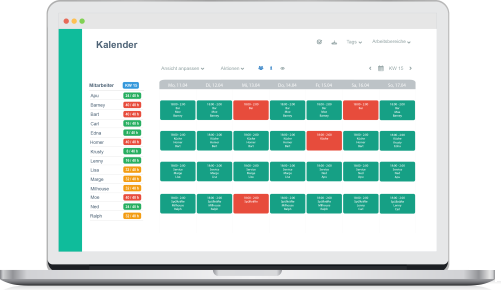
\includegraphics[scale=0.72]{images/lunchapp_mockups/mockup1} 
\caption[Mockup: Web-App]{Mockup: Web-App} 
\label{wamu1} 
\end{figure}

\begin{figure}[H] 
\centering 
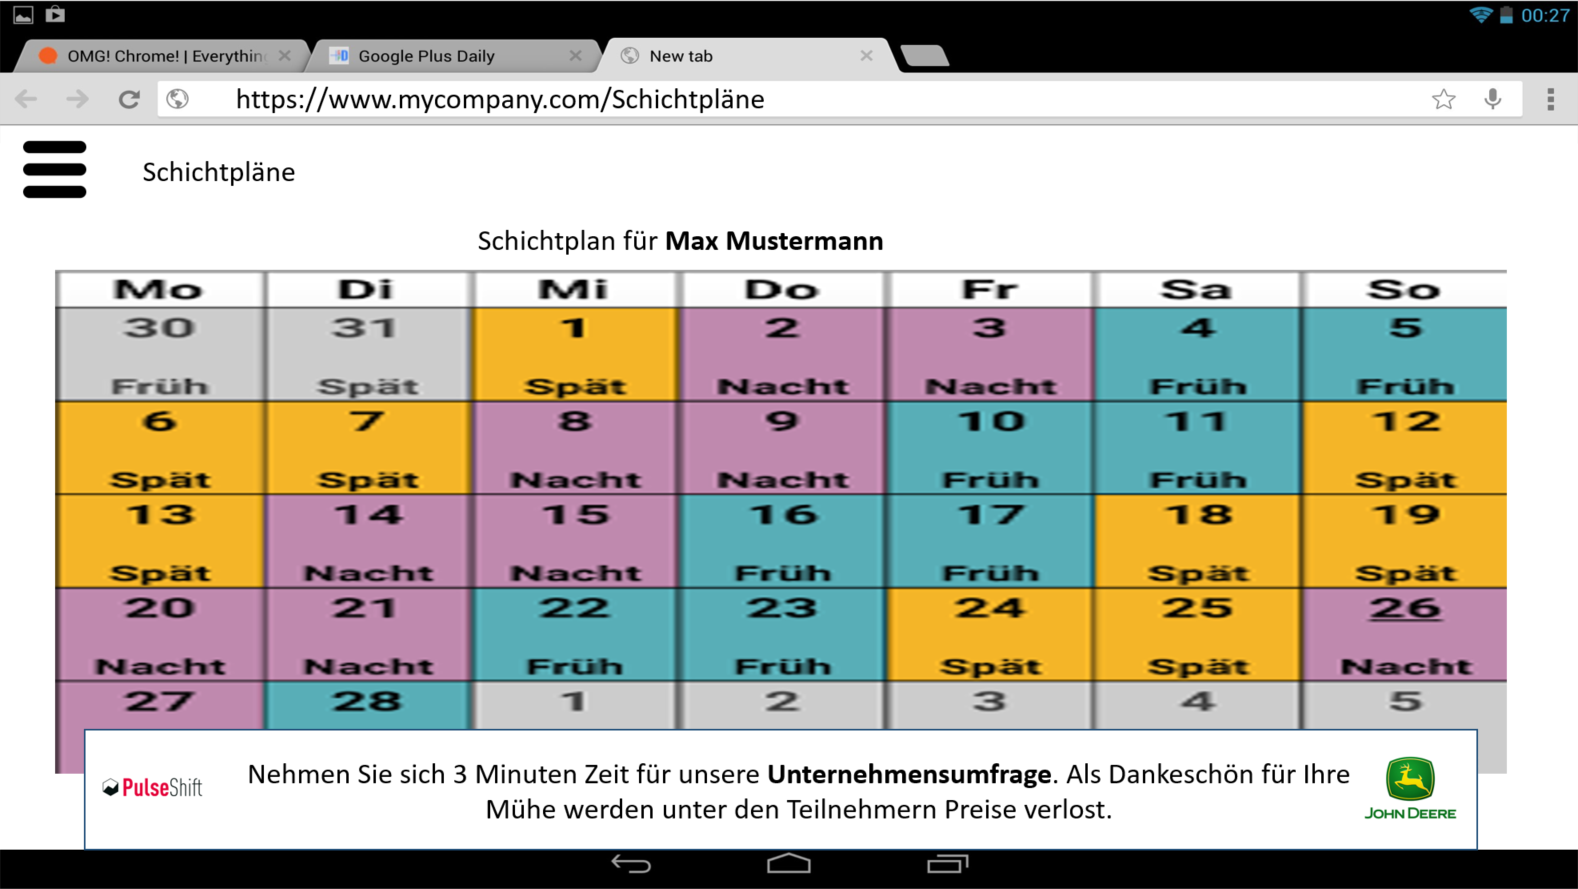
\includegraphics[scale=0.3]{images/lunchapp_mockups/mockup3} 
\caption[Mockup: Web-App mit Popup]{Mockup: Web-App mit Popup} 
\label{wamu2} 
\end{figure}

\begin{figure}[H] 
\centering 
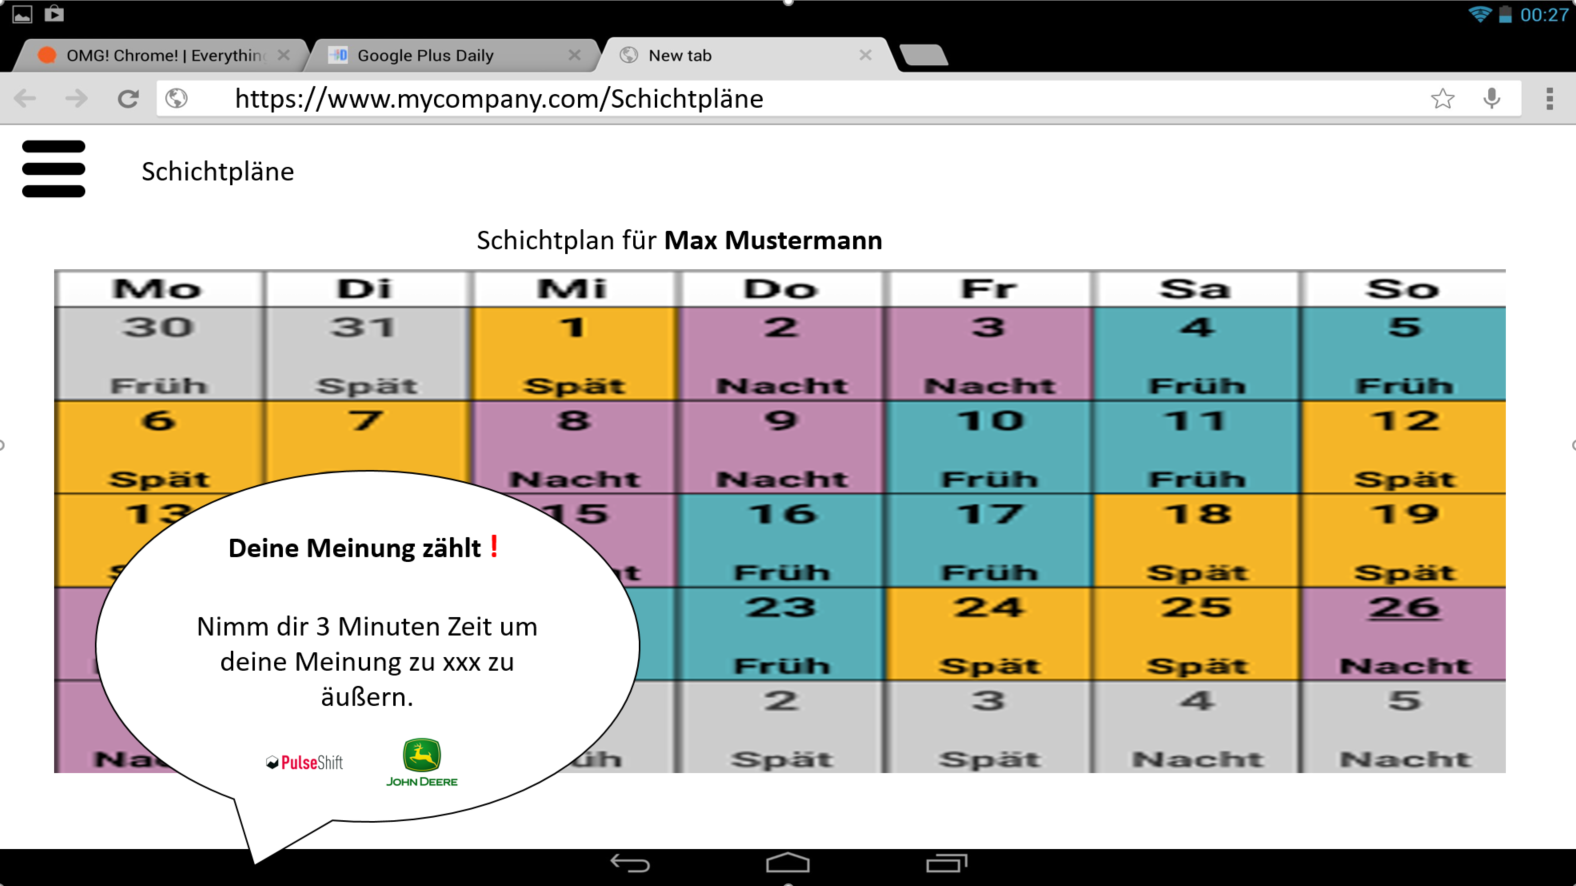
\includegraphics[scale=0.3]{images/lunchapp_mockups/mockup2} 
\caption[Mockup: Web-App mit alternativem Popup]{Mockup: Web-App mit alternativem Popup} 
\label{wamu2} 
\end{figure}



\subsection{Kostenfaktoren}

\paragraph{Initiale Kosten}
Bei der Erstellung der Webanwendung fallen einmalige Kosten an. Diese können unterschiedlich hoch ausfallen, je nachdem von wem sie durchgeführt wird. Ein wichtiger Aspekt bei der Erstellung ist die Implementierung eines sicheren Authentifizierungsmechanismus, um sowohl ausreichende Datensicherheit als auch Datenschutz zu gewährleisten. Die Kosten könnten daher zwischen 350 € und 1200 € liegen.

\paragraph{Regelmäßige Kosten}
Die Web-App muss fortlaufend mit den neusten Informationen versorgt werden und auf dem aktuellen Stand der Technik bleiben. Somit müsste es einen Mitarbeiter geben, der für die Instandhaltung und Aktualisierung der Seite verantwortlich ist. Dieser müsste schätzungsweise 8 Stunden pro Monat mit dem Aktualisieren der App verbringen, wodurch mit Kosten von mindestens 80 Euro pro Monat zu rechnen ist.

\subsection{Beurteilung des Projektteams}

\paragraph{Vorteile}
\begin{itemize} 
\item Der initiale Anreiz, die Webseite zu besuchen, wird durch die relevanten Informationen gegeben.
\item Es wird kein Druck auf die Mitarbeiter ausgeübt, sodass sie die Umfrage aus eigner Entscheidung starten. Somit sind die Umfrageantworten realistisch und qualitativ hochwertig.
\item Ist beispielsweise der Schichtplan die relevante Information und der Mitarbeiter ist mit seinem nicht zufrieden, könnte ihn das noch mehr anregen, an der Umfrage teilzunehmen, um etwas zu verbessern.
\end{itemize}


\paragraph{Nachteile}
\begin{itemize}
\item Es kann durchaus sein, dass die Mitarbeiter die Umfrage nicht nutzen, da sie keine Lust oder Zeit haben und nur die Informationen auf der Webseite einsehen wollen.
\item Dauerhafter administrativer Aufwand, da die Seite gut geschützt werden muss und die Informationen immer wieder aktualisiert werden müssen.
\end{itemize}


\paragraph{Bewertung und Potential}%$~~$\\
Das Kosten-Leistungs-Verhältnis ist hier in einem angemessenen Rahmen, daher sollte dieser Kanal weiterverfolgt werden. Die einmalige Implementierung erzeugt zwar erst einmal hohe Kosten, jedoch sind die laufenden Kosten relativ gering und können durch den Vorteil, die die Umfragen bringen können, aufgewogen werden.

\subsection{Feedback und Beurteilung durch PulseShift}

Von Seiten PulseShifts stieß die Single-Purpose-Web-App auf äußerst positives Feedback. Das Unternehmen erachtete für den Anfang eine hybride App oder progressive Web-App als sinnvoll. Der Vorteil einer solchen Lösung ist, dass plattformübergreifend Push-Benachrichtigungen unterstützt werden, beispielsweise dann, wenn dem Mitarbeiter eine neue Umfrage zur Verfügung steht. Bezüglich der konkreten Technologie gibt es seitens PulseShift keine Vorgaben. Jedoch soll die Umfrage, beispielsweise in einem iFrame, in die App gerendert werden können.


\subsection{Weiteres Vorgehen}

Für die Umsetzung haben wir uns zwei alternative Single-Purposes überlegt, die die Applikation dem Mitarbeiter bieten soll:

\begin{itemize}
\item Anzeige des Schichtplans eines Mitarbeiters
\item Anzeige des Lunchmenüs für verschiedene Kantinen und Wochentage
\end{itemize}

Beides bietet unserer Ansicht nach dem Mitarbeiter genügend Anreiz, die Anwendung regelmäßig zu nutzen und dabei gelegentlich an einer Umfrage teilzunehmen. Letztendlich haben wir uns für die Anzeige des Lunchmenüs entschieden, da viele Unternehmen die Schichtpläne ihrer Mitarbeiter aus Datenschutzgründen nicht an PulseShift weitergeben dürfen.